\documentclass[11pt,letter]{article}
\usepackage[top=1.00in, bottom=1.0in, left=1.1in, right=1.1in]{geometry}
\renewcommand{\baselinestretch}{1}
\usepackage{graphicx}
\usepackage{natbib}
\usepackage{amsmath}
\usepackage{gensymb}
\usepackage{hyperref}

\def\labelitemi{--}


\begin{document}
\bibliographystyle{/Users/Lizzie/Documents/EndnoteRelated/Bibtex/styles/besjournals}
\renewcommand{\refname}{\CHead{}}

\title{Climate Hazards \\ Log of meetings \& decisions}
\author{Lizzie, Isabelle Chuine, Ben Cook, Victor van der Meersch}
\date{\today}
\maketitle
\tableofcontents

\setlength{\parindent}{0pt}
\setlength{\parskip}{3pt}

\section{Meeting notes (including emailed discussions)}

\subsection{Montpellier June 2025!}

\subsubsection{2 June 2025: And we're back!}

Today we met in the afternoon and looked at my new heatmap (\verb|heatmapfitness.pdf|). We tried to summarize the results while staring at this with Isabelle helpfully pointing out that since mean results are already published/known we should focus on what the shifting variance does. 

\begin{itemize}
\item In almost all cases increased variance is bad, except for Fagus at 41 N and high warming where a little more variance means that chilling gets met now and again
\item Pinus has a veto where it does not get enough chilling, but once it does (lat 47 and 53) you see it follows the same trend where less variance is better
\item We discussed whether historical trends tell you what will happen with warming and basically we think they do -- both in trends and drivers, so I should check my old notes there!
\item If you think of fitness on y axis and some sort of thermal curve relativized for each species, the Quercus is on the left with warming increased performance, Fagus in the middle and goes either way (at the optimum, can get better or worse, depending on location) and Pinus in on the right --- just declining. 
\item I think I figured out that we looked at fruit maturation because we wanted to confirm it was doing as expected and not having a big impact on fitness ... I should update and close that issue. 
\end{itemize}

My to do items...
\begin{itemize}
\item Using our climate projections, what did we find out about climate change and variance (my recollection is that it goes all ways, but check)
\item Using printed heat map write out the drivers. 
\item What years are 0 warming?
\item Why does Quercus have more historical climate years than other species?
\end{itemize}

\subsection{What happened in September 2024 in Montpellier}

I worked on updating the endodormancy plots and leafindex plots that included freeze days and frost days (\verb|leafindex_decompose|). It's now mid-morning of my last day, so we'll see if I manage the fruit maturation plots also! UPDATE: finished the fruit maturation plots, info in issue \#13. 

I just met with Isabelle and Victor and these are the take-home messages:
\begin{itemize}
\item We are happy with Oct-Feb for the endodormancy plots  so I will delete the folder using Jan-Mar. I will make a few tweaks to those plots. 
\item The low leafindex values that we cannot explain are likely due to damage that we do not capture as I do not use the Leinonen (see 1996 paper) in my plotting. The actual equation is what PhenoFit uses and it allows hardiness to vary dynamically throughout the winter so those low days are probably due to the interaction of modeled hardiness and the minimum temperature.
\end{itemize}

\subsection{Overview of June 2024 in Montpellier}
This visit is when I finally did mean x var simulations -- did all warming levels and -50\% variance and +50\% variance. 
Also did ... Added flowering date and flower dormancy date to all figures. In the extras folder for now. 

Slightly larger topics we vaguely discussed. 
\begin{itemize}
\item Are there any general take-home messages from our simulations? Answer: Endodormancy and frost are key to predicting species responses to variance changes. Endodormancy response curves drive species responses so we need to get those right. 
\item How much do historical trends inform or help our understanding of simulation results?  Answer: Not much for variance, but some for warming. Basically, space for time is {\bf not great} for forecasting warming and useless for forecasting variance. 
\item How to slim all the work down to a `case study'?  Answer: Not possible, probably need to write as full paper, but I (Lizzie) still plan to step back and see if two papers are possible (one perspective and one data/research paper). 
\end{itemize}

\subsection{7 June 2024: Last day in Montpellier}
Met with Isabelle and Victor and discussed SD x warming results (I was a little exhausted so definitely not my best work, should check). Most notes in climhazardresults.pdf. 

We agreed we could: Drop latitude 47 from everything if we want. 

Also, temperature survival does not matter. At all. It does not matter in the model because the temperature for it is very low and by the time this temperature is hit, a species leafindex will have gone super low and leafindex trumps temp survival so temp survival does nothing. Isabelle said someday if she changed the model it could matter, but for now it is pointless (she added it originally because people said it mattered). We discussed this because I thought I saw perhaps a few more tempsurvival issues in the sd x mean runs (but did not check, these are just printed out to the screen in phenofitplotsims.R and phenofitplotsimsmeanvar.R), but given this does not matter, it does not seem worth checking.

Discussed FruitMat in depth, as it gets later or stalls with SD x warming. It has two curves, the first is sigmoid so unlikely to matter. The second is more interesting. I set up a git issue to work on plotting this. 

\subsection{4-6 June 2024: Victor and Lizzie}

\begin{itemize}
\item 4 June: We worked on climhazardresults.pdf! Including making predictions for mean warming x SD. \\
\item 5 June: Met with I\~naki \\
\item 6 June: Discussed predictions with Isabelle and Victor, including how important the endodormancy curves are to predictions. 
\end{itemize}

Isabelle mentioned Outi Savolainen paper showing trees are 100 years out of step with climate optimum; she said it was for spruce, but closest I found (on quick glance) was for Scots Pine \url{https://academic.oup.com/jhered/article/102/5/526/825887}.

\subsection{3 June 2024: Return to Montpellier!}

\begin{itemize}
\item Wrap up what is causing low leaf-index in Fagus simulations with SD (notes below).
\item Confirm which Quercus species set we wanted to use, there are three and (update) I am using the correct one which is \verb|Quercus_robur_ADuputie_Chuine.species|:
\begin{itemize}
\item \verb|Quercus_robur_ADuputie_Chuine.species| -- {\bf model I used for new sims (correct)} and assume we agreed to use (should check notes/git commits to make sure I updated all sims)
\item \verb|Quercus_robur_ADuputie_updated23June2023.species| -- model from Victor's approach I believe
\item \verb|Quercus_robur_ADuputie.species| -- first model we started with
\end{itemize}
\item Confirm I can ignore the drought and temp survival output -- yes, because we do not change the precipitation so drought survival should not vary with the simulations (and temperature survival is usually 1 -- since those values are rarely reached)
\item Go through SD sims again and make sure we understand all of them. (notes below)
\end{itemize}

Discussing SD results, including low leaf-index in Fagus simulations:
\begin{itemize}
\item While we think low leaf-index in Fagus simulations should be due to earlier budburst, the work from November to February suggests that it is cold temperatures in the winter. 
\begin{enumerate}
\item We discussed expand the window before leafout in my plots (\verb|leafindex_decompose_Fagus.pdf|), but then the temperature I am using as a low may be too high. This interplay between cold hardiness and frost is cool, but hard to evaluate given current model output.
\item Relatedly, delayed dormancy break date should keep hardiness higher longer, but we still see more frosts. 
\item I should count up the days below a species' max tolerance.
\end{enumerate}
\item Remember: Leafindex generally declines because of frost, this leads to declines in MatIndex. Low FruitIndex comes from frost on flowers.
\item Quercus shows similar Leafindex to Fagus.
\item Pinus shows delayed dormancy break which leads to later leafout (other species have delayed dormancy break date but does not lead to later leafout). 
\item A lot of sims should delayed dormancybreak date so we talked alot about visualizing this more. 
\end{itemize}


Other notes: Victor and I discussed what's the simplest process-model for SDMs and he mentioned TTR SDM (but it sounds more like a correlative SDM than a real process model, so I should look into it more).


\subsection{3 January -- 27 February 2024: Understanding low leaf index in \emph{Fagus}}
\emph{Lizzie wrote this up on 1 June 2024: Yes, big gap due to teaching through April and then visiting Zurich in May. But, here we are.}\\


From Victor on 27 February: 2024
\begin{quote}
From what I can see in the trace:

Year 1952:
\begin{itemize}
\item a hard frost event happened on April 2nd (DOY 93, leap year), with a Tmin = -11 (min Tmin in the year = -16, Nov. 17th) $\rightarrow$ leaf index dropped to 0.48
\item it was 24 days before leaf unfolding date (April 26th, DOY 117)
\item the day before (DOY 92), the Tmin = -7 did not have any effect... I guess the bud cold-hardiness state was enough to resist to -7 but not to -11?
\end{itemize}

Year 1955:
\begin{itemize}
\item an extreme frost event happened on Feb. 17th, with a Tmin = -18 (min Tmin in the year = -23, Feb. 23rd) $\rightarrow$ leaf index drop to 0
\item it was 83 days before (potential) leaf unfolding date (May 10th, DOY 130)
\item the maximum frost resistance for Fagus is -20, so at -18/-23 injuries must occur... 
\end{itemize}

In these two examples, frost happened several weeks ($>$15 days) before leaf unfolding (up to 83 days!).
In the first case, in early April, I guess we can still talk about a `late spring frost.' 
But in 1955 it seems to be more related to hard conditions during winter. 

So it makes sense you did not see anything $\pm$15 days before leafout...
\end{quote}

And I replied to Isabelle (26 February 2024, with 3 files: \verb|leafindex_decompose_Fagus.pdf| and \verb|fit4Trace_loc_1_pheno_1954.txt| and \verb|fit4Trace_loc_1_pheno_1951.txt| and ):
\begin{quote}
I increased the days to look for frost to ±$\pm$ 7 days before leafout 
(results attached) and tried $\pm$ 15 days (not shown but it added a couple 
more frost days=1 but not so many to explain things). Each of these 
picks up more frost days, but not so many. I have also plotted the 
dormancy break date.

None of these seemed insightful to me, so I have attached trace plots 
for the requested location and sims, for two years.
\end{quote}


Isabelle replied (16 January 2024):
\begin{quote}
We look at your figures with Victor yesterday. The decrease of the 
LeafIndex cannot be due to something else than increased frost damage 
but it is difficult to show it on a simple graph because frost damage 
depend on the development of the buds and the temperature and 
daylength conditions with a memory effect. What is strange though is 
that you see no frost days (Tmin$<$5.3C) within 7 days after BB in any 
case while sometime the BB is 30 days earlier than normal. Two ideas:

increase the window around BB $\pm$ 7 days, $\pm$ 15 days

Look at the dormancy break date.

Last option is to look at a Trace for one site and one year for $+$50\%  sd for sim53
\end{quote}

On 3 January 2024 I emailed: 
\begin{quote}
We discussed getting the number of frost days and late leaf unfolding days, especially for Fagus ... (See file: \verb|leafindex_decompose_Fagus.pdf|) I used the FHminfe value (-5.3) and counted up days $<$FHminfe the day of and 7 days
after leafout. 
\end{quote}


\subsection{9 December 2023:  My notes on scheduling and cleaning up folders}
Isabelle is free in May, but Ascension is the second week (though now it seems that I am busy in May); she is probably away first and second weeks of June. So options might be April 29-2 May (week before is 22-26 April) or 17-21 June.

In cleaning up \verb|climhazards_QuercusUpdatedModel.pdf| I kept referring to our new parameter file as 'ending in updated23June2023' but that was the very first parameter change file we tried. When I opened PHENOFIT I was using the species file added in November 2023 (ending in `Chuine') and the trace files we kept are also using this new file, so I updated my language throughout the document. 

\subsection{3 december 2023: Good ref}

From wheat paper by I\~naki and colleagues: ``Tillering stands out as the most resistant with the lowest mean threshold. These results are in agreement with previous studies showing that the reproductive stage is more sensitive to cold stress than the vegetative stage (Manasa S et al. 2022).''  Manasa S, Lekshmi, Madhusmita Panigrahy, Kishore C. S. Panigrahi, et Gyana R. Rout. 2022. Overview of Cold Stress Regulation in Plants. The Botanical Review 88 (3): 359‑87. \url{https://doi.org/10.1007/s12229-021-09267-x.}
% \section*{Some current issues}

\subsection{17 novembre 2023: Meeting at CEFE with Isabelle} % Victor away

{\bf We agreed to do mean x SD simulations of the following:} All warming (my idea, it's easy and helps you see the pattern) x SD decline of 50\% and SD increase of 50\%. We think this is the best way to understand what we find. 

We also discussed re-arranging the plots of all metrics (e.g., \verb|meansim47_allmetricsFS.pdf|): 
\begin{itemize}
\item Remove drought and temperature survival if they never change?
\item Add flowering date and flowering dormancy date perhaps?
\item Row 1: fitness, survival, fruitindex, matindex
\item Row 2: Carbon, leafindex, dorm break date, leaf unfolding date
\item Row 3: Drought survival, fruit mat index, fruit (can't read: le nes?), temp survival
\end{itemize}

\emph{Other notes from today:}

Relevant reference: Caignard et al. 2017 (Sci Reports).

For Pinus at southern site, see `Scots Pine' discussion in Duputie. At 47 N, warming leads to same effect as at southern site (carbon survival due to late leafunfolding).

FHminfe -- this is the minimum temperature for no leaf damage after budbreak, check in any species file for this. The only other way to get a low leafindex is when the leaves do not unfold (leadunfoldingdate of 365). Need a plot that shows leaf unfolding date and the number of frost days together. \\
FHminfl -- this is the minimum temperature for no flower damage after budbreak, check in any species file for this.\\


\subsection{16 novembre 2023: Meeting at CEFE with Isabelle \& Victor}

We spent the morning talking about Victor's very cool project on forecasting the Holocene, then spent the afternoon on the new results from new parameter set for Quercus. \\

See \verb|climhazards_QuercusUpdatedModel.pdf| for more on the results of the new parameter set. Related to this, we checked if the PET adjustments were okay (see \verb|testpetoutput.R|... why? I cannot recall, but we were worried about them) and they seem fine. 

I also added the curve for the f(x) to the pinusflowerendodorm.pdf figure (ignore the height of the curve) so we could better see the f(x) versus the temperatures. 


\subsection{15 novembre 2023: Meeting at CEFE with Isabelle \& Victor}

To do ...
\begin{enumerate}
\item Use the new parameter set for Quercus from Victor. It is based on expert opinion, whereas the one I have now is based on inverse calibration. 
\item Fagus simulations future -- to look at LeafDormancyBreakDate -- calculate the mean C 1 Nov to 1 Fev for 41 N site (we expect it to be around 13 at 0; and a little less than 13 at reduced SD), and for the other sites -- we expect more days above 13 with higher SD in all sites. 
\item And for Fagus, get the number of days in the week after leafunfolingdate below -5.3  (freezing for leaves near the time of leafunfolding date, there's a different temperature for further before leafunfolding date.) {\bf Should try to functionalize this to work for other temperatures and other temporal windows.} % <FHminfe>-5.3</FHminfe>
\end{enumerate}

Notes during meeting (in addition to to do above):
\begin{enumerate}
\item Remember:
\begin{enumerate}
\item Drought survival uses only precip; but fruit maturation depends on precip-ET
\item FruitIndex is affected by flower development (frost on flowers will reduce fruit). 
\end{enumerate}
\item With mean warming the effects -- and their drivers -- depend on where you start (with latitude). With SD the results and drivers are very similar (expect the effect on whether leafunfolding date gets later depends on latitude, likely because further north the later leafdormancy break date happens when it is too cold to unfold): leafdormancybreakdate gets later and likely drives more frost (need to check, see above task); leafunfoldingdate also gets more variable consistently. Note: MaturationIndex depends on LeafIndex. 
\end{enumerate}


\subsection{14 novembre 2023: Prep for meeting at CEFE this week (may want to revisit in 2024)}
These are my notes before the meeting; I updated them on 9 December 2023. 

\begin{enumerate}
\item Need to review our simulation findings -- most notes are in 23 juin 2023. (We did this.)
\item Are we happy with the \emph{Quercus} parameters? 

We now use \verb|cmaes fit subset2_rep2.species| which is the full updated parameter set (not just the leaf and flower parameters)? (Answer was no; we fit a new version that we will go with.)
\item Check my notes on Pinus results below with Isabelle. (Done, but I still need to review Scots Pine in Duputie paper)
\item Review results with future sims -- agree we can ignore calendar issue (and just toss plots in supp)? (I think we can ignore it.)
\item Decide on SD and mean for one run with both ... do it, and interpret it. Do we have any predictions? (Done.)
\item Which figures? Question: What do we want to present? We have a lot .... (NOT done.)
\item Start writing up section on PHENOFIT so we can agree on it.  (NOT done.)
\item Questions for colleagues file. (DONE)
\item Smaller items
\begin{enumerate}
\item We will skip changing WHC, right? (This came up again when looking at results; basically was left up to me to decide as it is more work. Notes are in \verb|climhazards_QuercusUpdatedModel.pdf|
\item I should write up the METHODS before I go, including: (NOT done.)
\begin{enumerate}
\item Penman-Montieth
\item Where we got the species parameter files
\item Where the climate data comes from.
\end{enumerate}
\end{enumerate}
\end{enumerate}

\subsection{25 September 2023: Email from Victor about how many days are in a model year...}
Victor wrote:
\begin{quote}
I also forgot to tell you that not all models have the same calendar:\\
- IPSL, MPI and MRI have a gregorian (``true") calendar, with either 365 or 366 days\\
- GFDL has a 365-day calendar (no leap year)\\
- UKESM has a 360-day calendar (12 months of 30 days each)\\

Most of the time, February 29 is interpolated from February 28 and March 1.\\
For 360-day calendar, it is a bit more tricky. I've seen three different approaches:\\
- insert a new day every 72 days in order to add 5 days in a year - this new day is randomly selected in the 72-day block\\
or\\
- drop Feb. 30 and 29 (except in leap years), and interpolate 31st of Jan, Mar, May, Jul, Aug, Oct, and Dec from the days before and after\\
or\\
- directly interpolate one day every 72 days (and Feb 29 when needed)\\

Anyway, I think in our case we can keep the model initial calendar, but we may want to adapt your monthly calculations?\\
If you prefer, I can also send you the data with interpolated extra days (when needed).\\
\end{quote}

\subsection{24 September 2023: No meeting, just work notes}

No meeting, but I feel like some notes would be good as I fall out of practice on this project.... \\

The pressing to-do is checking the projections so we can use them to estimate our shifts. I received the updated (now including historical period) SSP2245 from Victor, but only have tmin as best I can tell and I could use a higher scenario. I did update the code though today to look at the historical data versus {\bf one} (for now) GCM and I am sending that on to Victor and Ben.\\

\subsection{9 August 2023: Emails from Ben \& Victor about projections}

Victor wrote:
\begin{quote}
You may find further information in this paper, where they first downscaled projections using the ERA5 reanalysis (coarser resolution than ERA5-Land they now use).
In particular, figure 4 (right panel) gives an idea of the difference between ERA5 reanalysis and downscaling results.

\url{https://doi.org/10.1016/j.dib.2021.106900}
\end{quote}

And Ben replied:
\begin{quote}
I looked through quickly, but nothing seems to be particularly odd here. You can kind of see in the first linked paper how, even in the downscaled data, the extreme ends of the PDFs extend a bit further in the models than in the observations (Figure 2). This figure is for the whole globe, so I would expect these minor difference to be larger at small scales.

As I mentioned yesterday, I think it would be good to compare the observed time series to the historical simulated time series, and also just stitch the historical and projection data so that we can see how everything looks at once. 
\end{quote}


\subsection{8 August 2023: Meet with Ben Cook}

\emph{First we discussed what to do with the model projections data and how to decide if it is okay to use}

I should do a moving average and STITCH projection data together with the historical data. \\

This is a LOW warming scenario; better to look at the 7.0 scenario (or the highest scenario we can get) and see if the warming signal gets stronger. \\

Noise in the models is higher than historical models, but maybe not so bad.... \\

Initial conditions should be end of historical simulation (so should be 2015). \\

Get more info on the downscaling (just a bias correction? Or did they also scale the variance?). \\

Also, we're looking at individual grid cells, so the re-analysis (historical) product could be smoothing things spatially in a way the model data is not smoothed (for example, the historical data may be smoothed through local stations). You could check for this by correlating with nearby grid cells and map the correlations to see if the re-analysis (historical data) is more correlated across space than the model data. \\

Could also plot the overlapping historical period and model period (if they provide those from the models). \\

If it works and we want to use the model forecasts, you do model averaging as the last step. \\

Basically four scenarios:\\
2.6\\
4.5\\
7.0\\
8.5\\

\emph{Then we discussed which scenario is realistic.} 

When Ben says `we're on track for 4.5' he is referring o the `policies and action.' Before Paris Agreement when there was no international agreement, the worst case scenario (8.5) seemed more possible, but it now seems unrealistic to think we will keep it under +2C by 2100 but also equally unlikely that we will hit 4-5C by 2100. He thinks of 2C and 4C as reasonable best and worse scenarios and we should be communicating those options. \\

Discussion of the action tracker webpage (CAT thermometer):
\begin{itemize}
	\item  Blue is polices and action -- what is happening now, based on our best guess of current policies. You can check compliance information. 
	\item The other colors are planned policies. 
	\item In blue and purple (less aspirational ones) the climate keeps warming after 2100.
\end{itemize}

\subsection{18 July 2023: Email from Victor with projections methods}

Here's the paper associated with future climate simulations : \url{https://doi.org/10.1016/j.dib.2022.108669}

It has been done by researchers from IPSL, a research institute which develop one of the GCMs included in the CMIP6 (IPSL-CM6A-LR).
I chose these data as they were downscaled with ERA5-Land data - and thus it should be coherent with the data we used for PHENOFIT simulations.

\subsection{14 July 2023: What I have done recently}
I ran two versions of a new Quercus model (first just changing the leaf model, then using a whole new parameter set from Victor). See \verb|climhazards_QuercusUpdatedModel.pdf| Isabelle wrote (and I agree):``The new results with Victor-CMAES parameters make more sense actually than Duputie parameters and surely there is something to dig into there for Victor and me related to his PhD project." So I will move forward with these results. 

I also looked at whether flowering dormancy for Pinus could be driving some of the temperature variance results (see pinusflowerendodorm.pdf and pinusflowerendodormMeanTemp.pdf) by estimating flower endodormancy (Isabelle sent the function and I pulled the parameters). Looking at this Isabelle explained:

\begin{quote}
What I see is that more variance generates more days that fall out of the range of optimal chilling which is ~between -5 and 0°C for the parameter set of Pinus of Duputié, so chilling accumulation slows down and dormancy break date is delayed. 
\end{quote}


\subsection{23 juin 2023 with Isabelle \& Victor}
{\bf Last day in Montpellier!} With Victor and Isabelle, we went through results to date:

We reviewed first the historical results, see Fig. \ref{fig:historicalfitnessl}. 

Next the mean warming simulations. In understanding \emph{Fagus} results (Fig. \ref{fig:fagusmean3}) we discussed how we could see that at low latitudes (Fig. \ref{fig:fagusmean41}) that there was reduced CarbonSurvival (not enough cold means late dormancy) and thus FruitMaturationDate gets later. While at higher latitudes (Fig. \ref{fig:fagusmean53} ) there is an increase in the FruitIndex as FruitMaturation is higher. 

I should review the \emph{Pinus} results in Duputie et al. 2015. For our mean results, it looks like carbon could be the issue again. 

For the mean results for \emph{Quercus} we wondered whether the Leaf model parameterization was driving the results. It's currently set to have a -4.5 maximum temperature. To check this we created an updated file (\verb|Quercus_robur_ADuputie_updated23June2023.species|) using the leaf model parameterization from Van der Meersch \& Chuine 2023 (\verb|cmaes_fit_subset2_rep2.species|). I need to run this new model parameterization.

Then we reviewed the SD sims. I took less notes, but there was a fair bit of similar drivers for each species (e.g., for \emph{Fagus}, which is more frost sensitive we see lower LeafIndex at the higher latitude models likely due to frost) but also a lot of discussion over the balance of where higher SD would put some of the non-linear curves. 

\begin{figure} 
 \begin{center}
\noindent 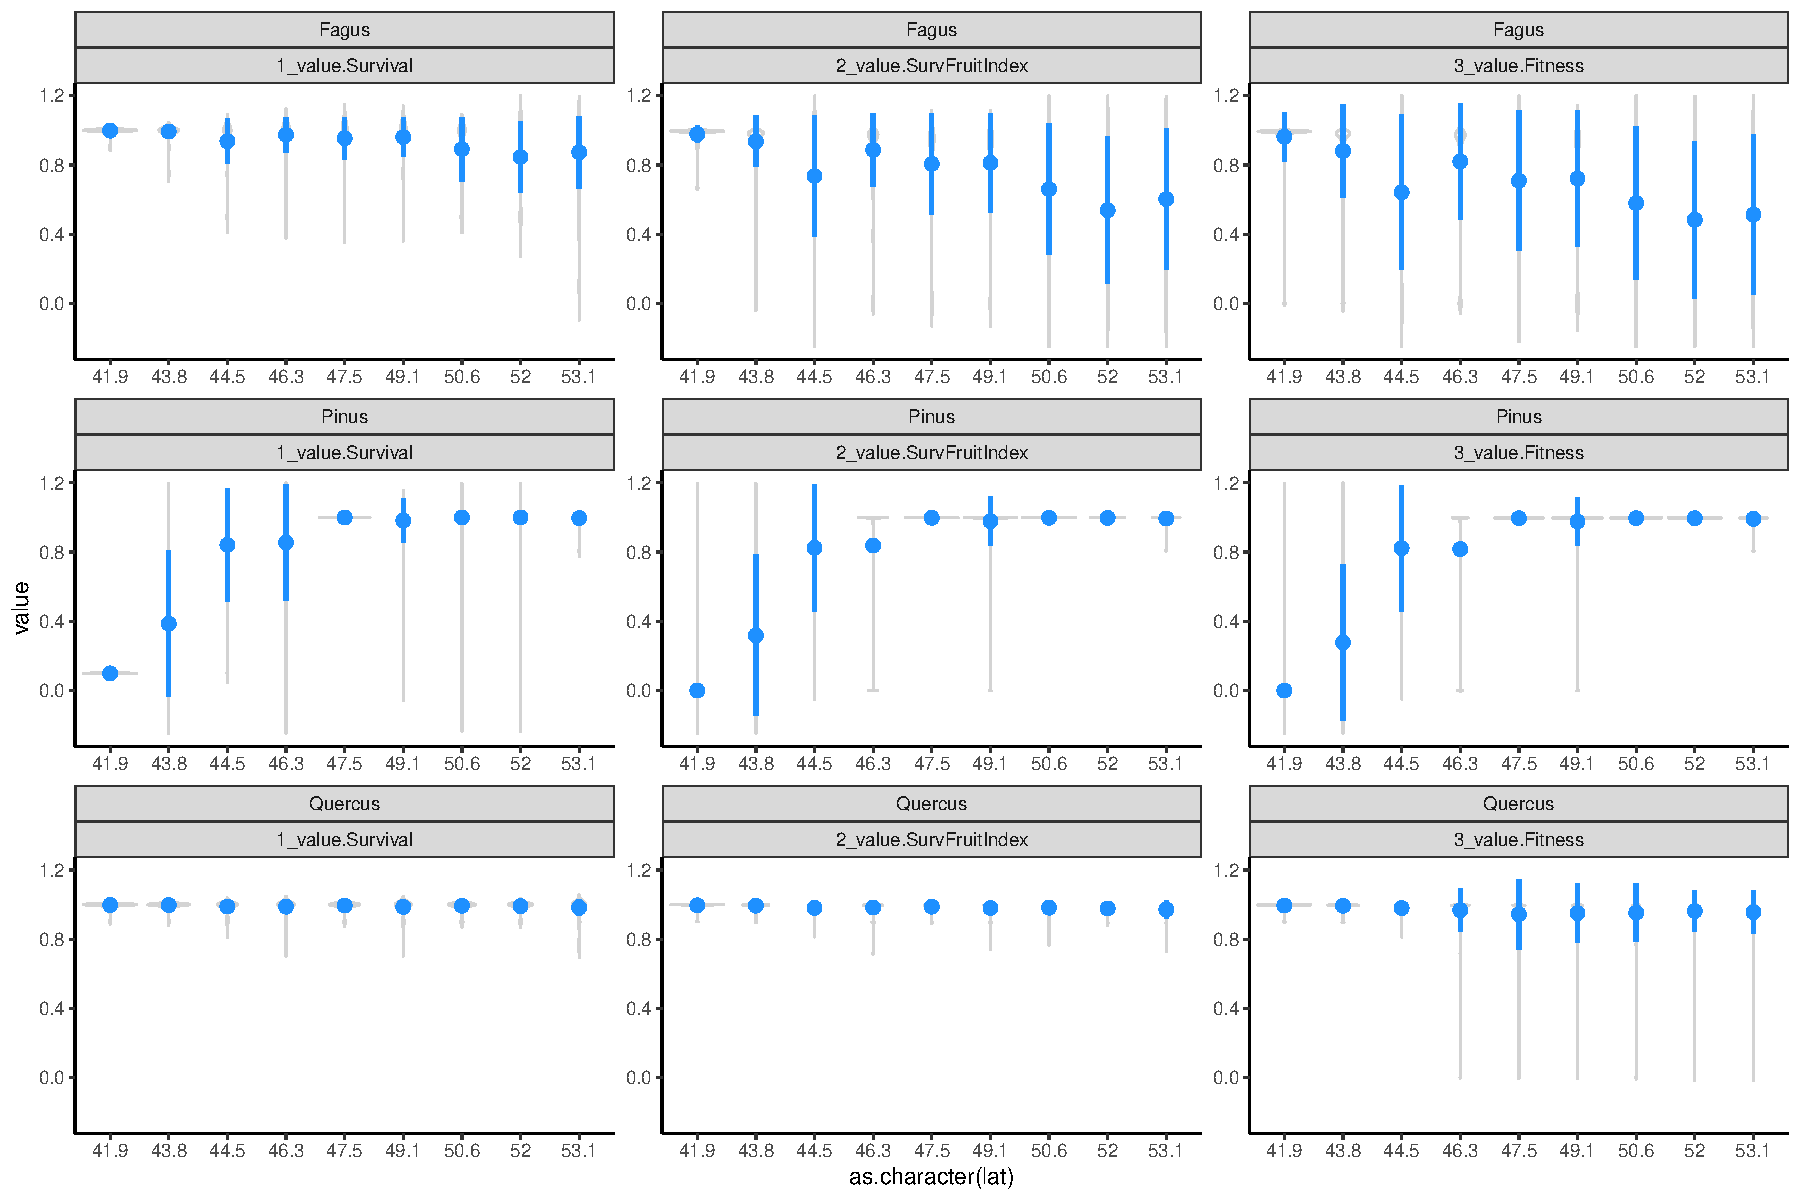
\includegraphics[width=1\textwidth]{..//analyses/graphs/phenofit/historical/fitnessBuildup.pdf}
  \caption{These results build through the multiplicative components of fitness (which are multiplied together): Survival (left), Survival$*$FruitIndex (middle) and Fitness, which is Survival$*$FruitIndex*MaturationIndex (right). Given high survival and little change between the middle and right panels we can see that \emph{Fagus} is determined mainly by FruitIndex (this makes sense as it is often affected by frost damage, having a low tolerance of low temperatures). We see next the for \emph{Pinus} survival dominates (often it does not meet the chill requirement for leafout and thus has no carbon and low CarbonSurvival so low total Survival) and finally, for \emph{Quercus} it's MaturationIndex (this makes sense as the fruits are quite large and can take a long time to mature---it doesn't always happen according to this model). }
  \label{fig:historicalfitnessl}
  \end{center}
\end{figure}


\begin{figure} 
 \begin{center}
\noindent 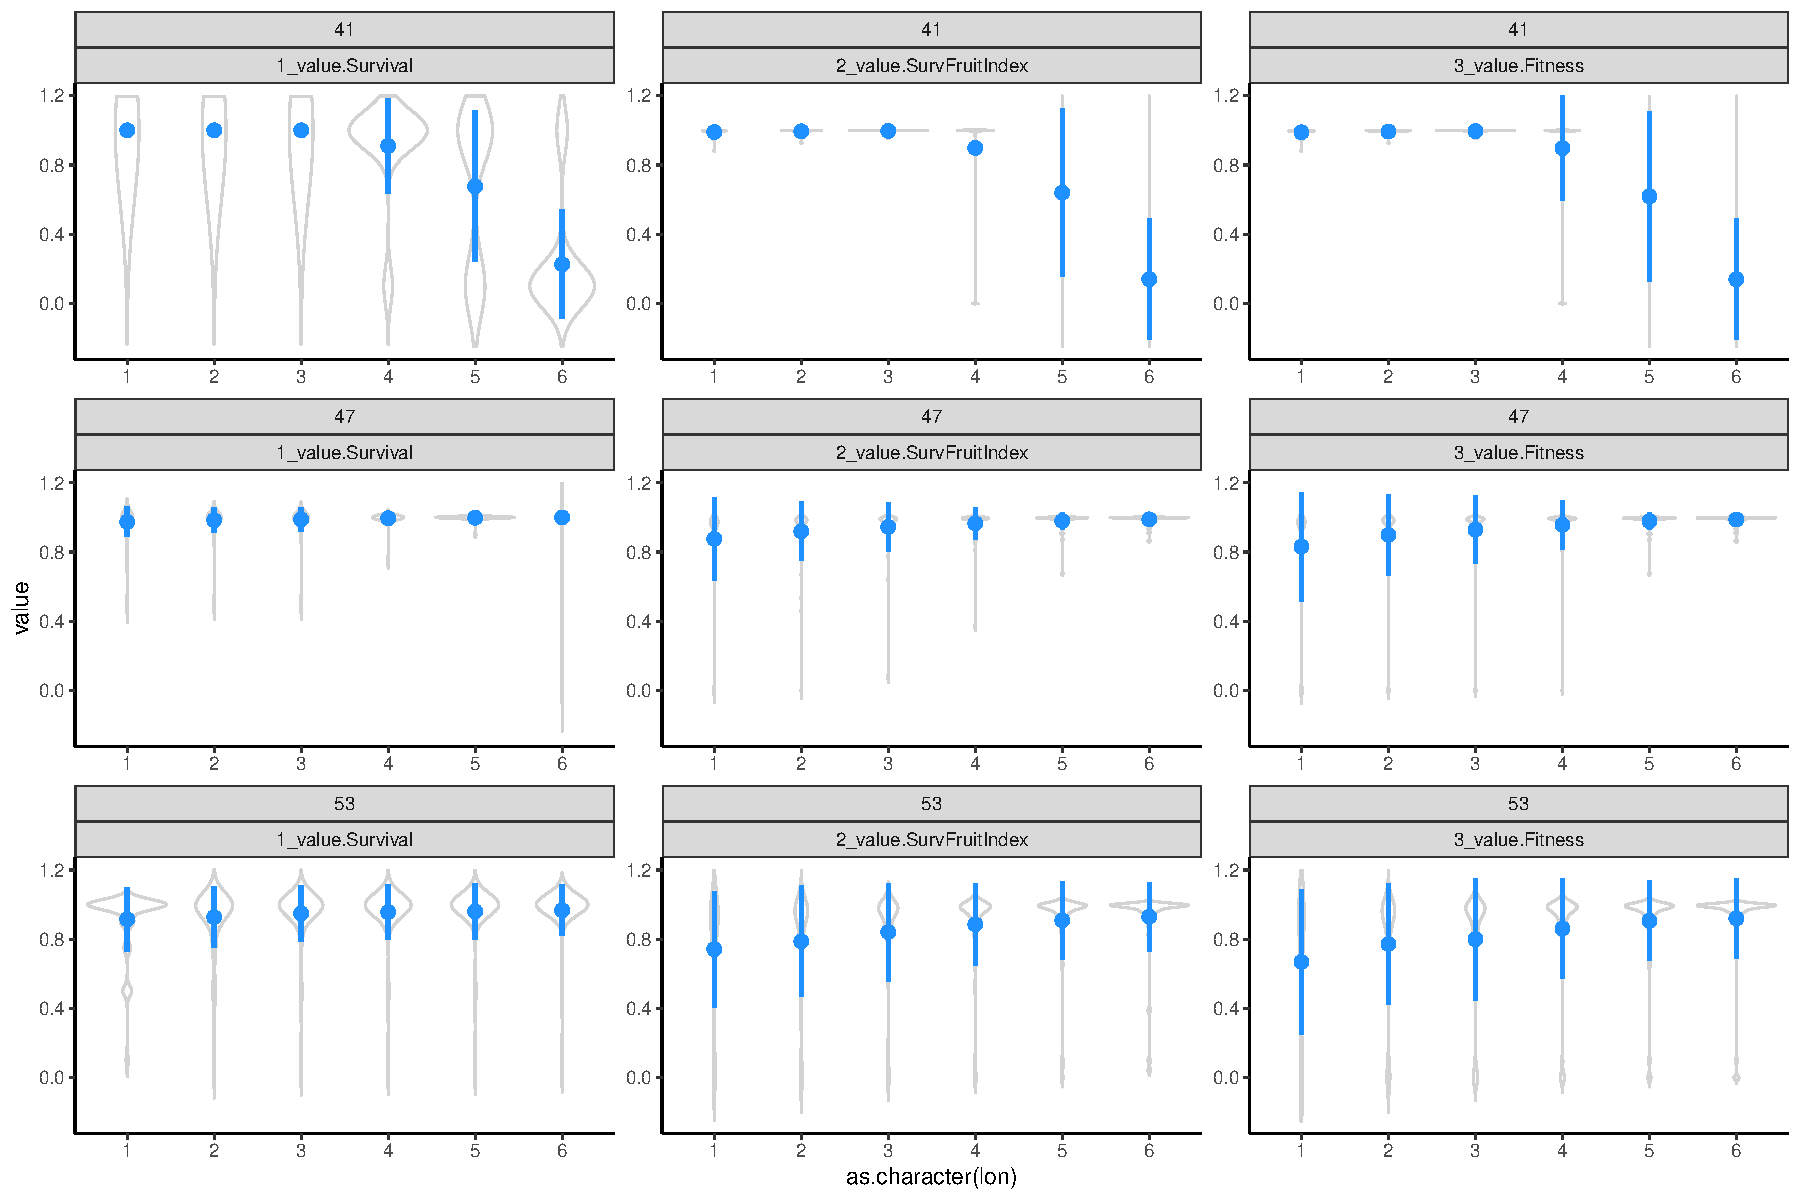
\includegraphics[width=1\textwidth]{..//analyses/graphs/phenofit/sims/metrics3/meansim_3metricsFS.pdf}
  \caption{\emph{Fagus} across 0 (1) to $+$5 (6) meaning warming showing three latitudes. In June 2023, we discussed: at low latitudes (see next figure) that there was reduced CarbonSurvival (not enough cold means late dormancy) and thus FruitMaturationDate gets later. While at higher latitudes (see Fig. \ref{fig:fagusmean53}) there is an increase in the FruitIndex as FruitMaturation is higher.}
  \label{fig:fagusmean3}
  \end{center}
\end{figure}

\begin{figure} 
 \begin{center}
\noindent 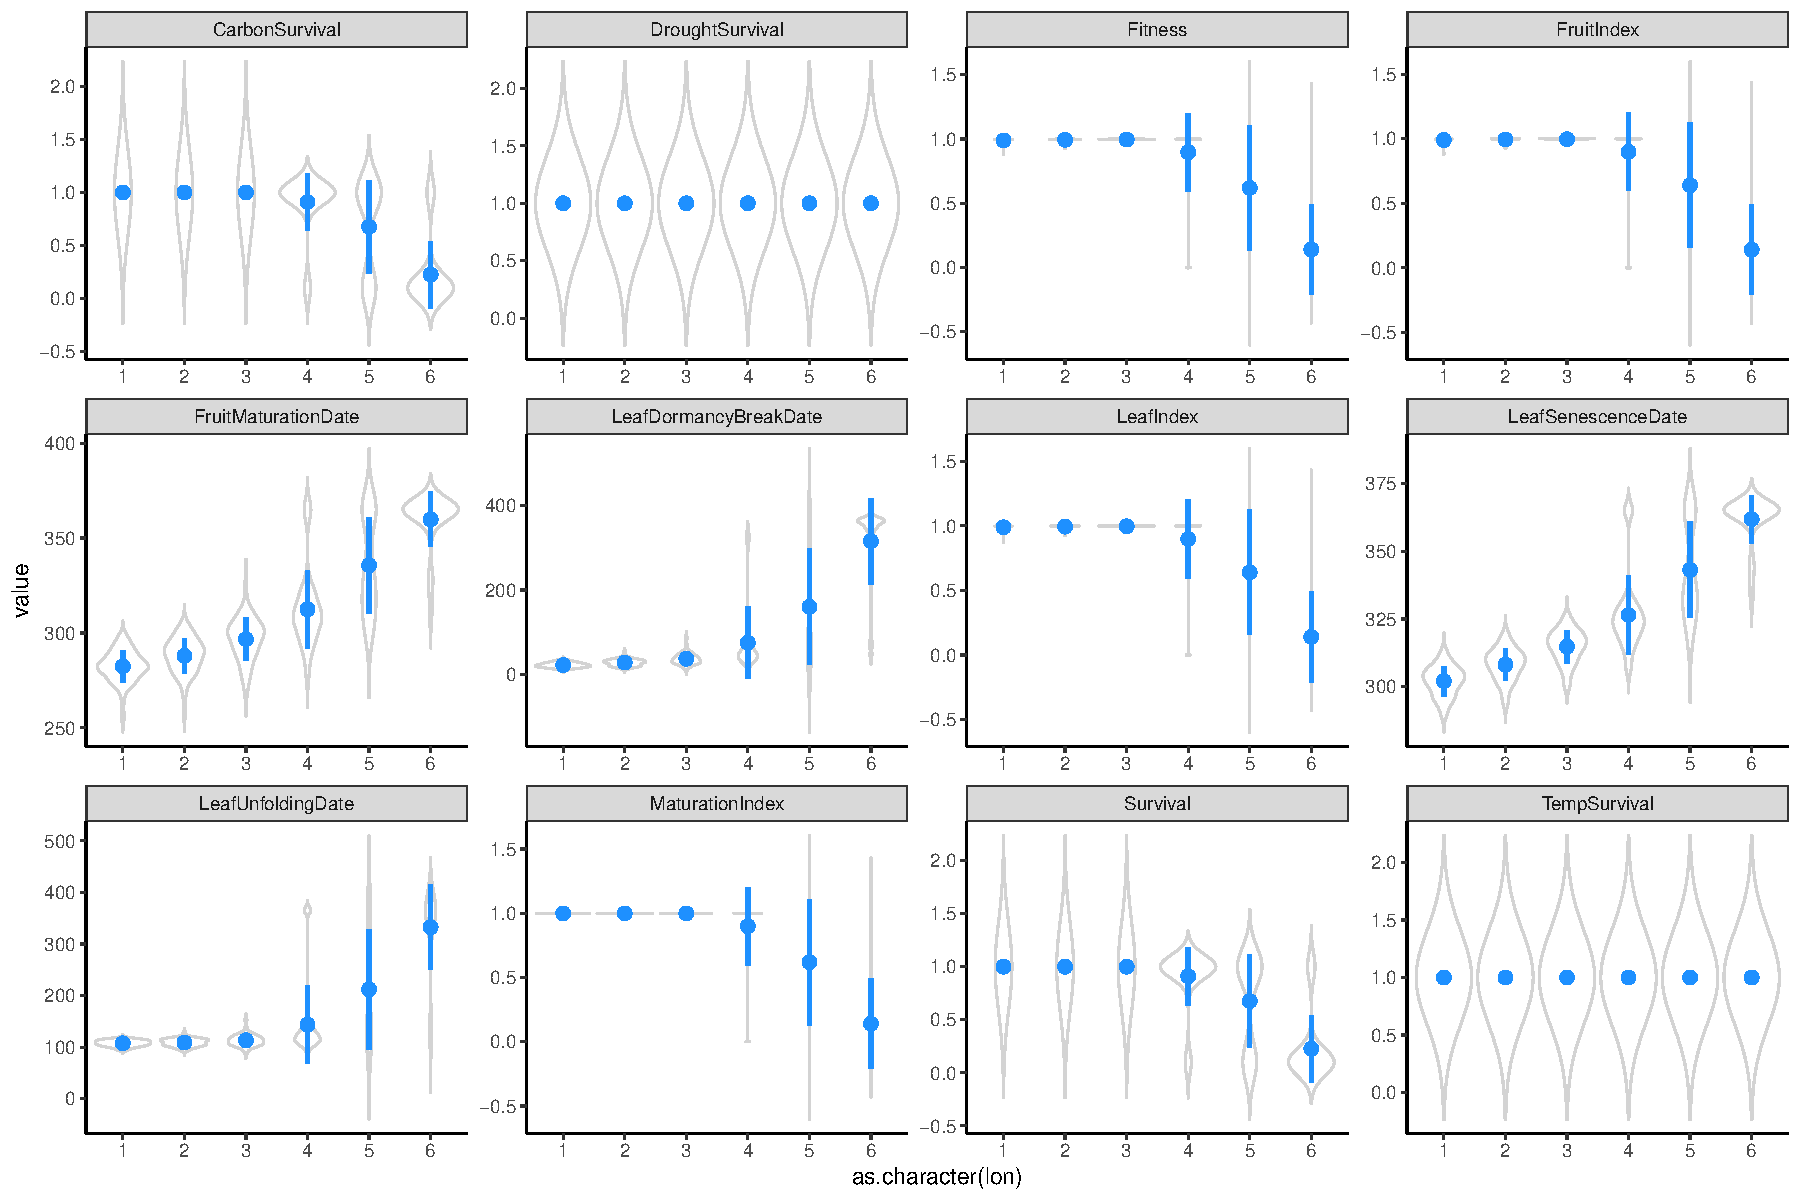
\includegraphics[width=1\textwidth]{..//analyses/graphs/phenofit/sims/meansim41_allmetricsFS.pdf}
  \caption{\emph{Fagus} across 0 (1) to $+$5 (6) meaning warming across fitness components at 41 latitude. Low fitness is driven by low carbonsurvival, which occurs because of late dormancy break date (because leafdormancybreakdate is variable that's the driver; if it were frost, we'd see more constant leafdormancybreakdate and variable in leafindex).}
  \label{fig:fagusmean41}
  \end{center}
\end{figure}

\begin{figure} 
 \begin{center}
\noindent 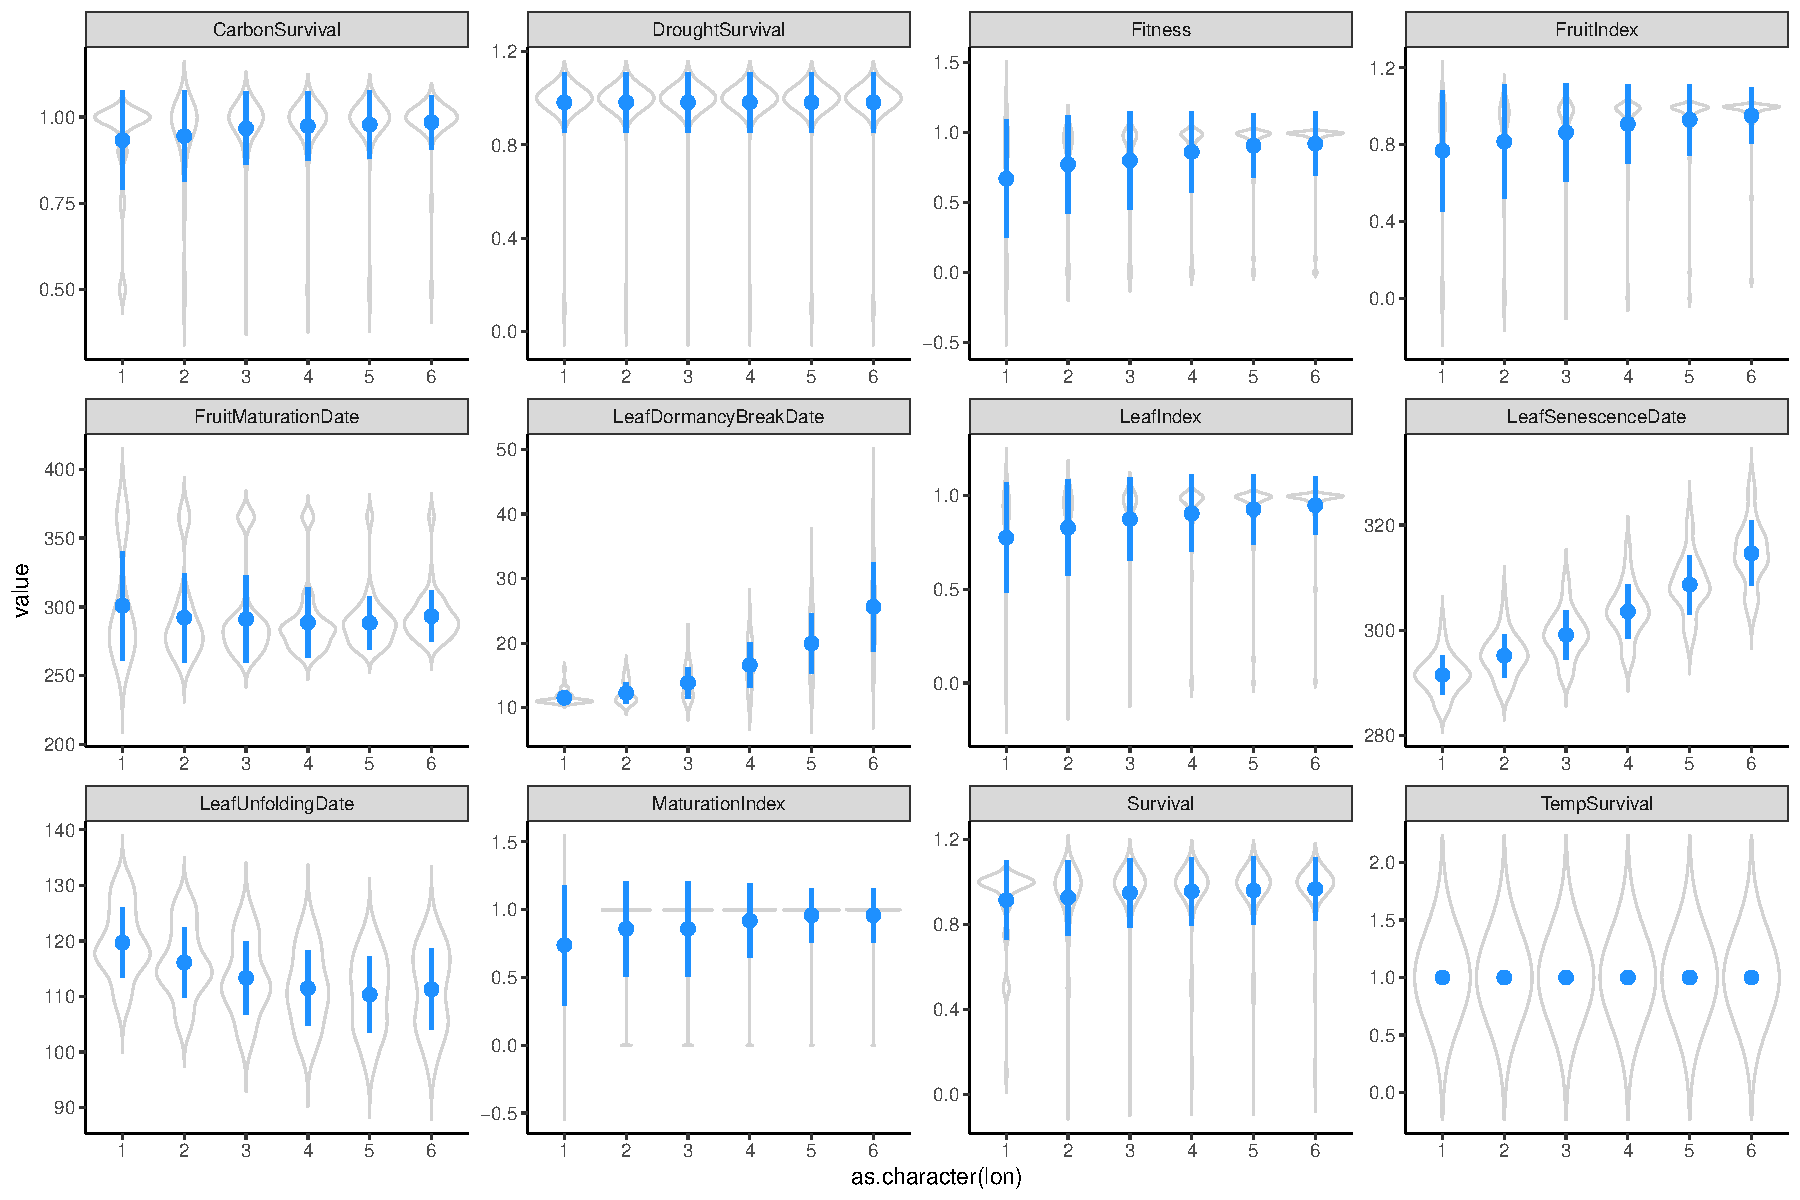
\includegraphics[width=1\textwidth]{..//analyses/graphs/phenofit/sims/meansim53_allmetricsFS.pdf}
  \caption{\emph{Fagus} across 0 (1) to $+$5 (6) meaning warming across fitness components at 53\degree N latitude. Here's warming reduces frost and thus fruitindex goes up and survival goes up. Note that the leafdormancybreakdate also gets a little later but leafunfolding does not because the warming is still enough for get earlier leafout (and there is a buffer where early dormancybreakdate does not matter because it's too cold leaf unfolding to start. }
  \label{fig:fagusmean53}
  \end{center}
\end{figure}

\subsection{22 juin: Stuff I did today \& chatting with Victor}

Discussed authorship with Isabelle, she does not care too much, but in her lab she usually puts herself last. 

Using Victor's nice file, I updated my code the PET is adjusted depending on temperature. On quick glance, it did not do much. But Victor and I checked and it did impact FruitIndex, which was expect (not DroughtIndex as also expected). 

I tested whether increasing SD in a simple threshold model should make the leafout date earlier. Answer is no. 

Victor does not use GUI for PHENOFIT, so someday I should probably switch to doing it without the GUI for safety? Especially if doing many rooms. 

Drought effects are separate from temperature effects; no interaction... Isabelle thinks they are multiplicative effects. Limit for growth is 0.4 relative extractable water for all C3 species. Isabelle will send the reference. 

\emph{Victor}:
PET should effect FruitIndex (and it does! Phew). It should not effect DroughIndex in PHENOFIT4 (also appears true). I compared between the PHENOFIT output before fixing PET and after. \\
It looks like the fixed dates for PHENOFIT must be the same date for all years, to discuss with Isabelle.\\

\subsection{20 juin with Victor \& Isabelle}

Today we agreed to focus on mean shifts (0-5C over baseline) and variance shifts (need to look at at data but should do lower and higher) and then we could someday later put together a FEW of the combos, but not all of them (not the full factorial I have been coding; this is sort of a relief as we have a lot going on). 

Maybe don't change the WHC, if we are interested better to change the precipitation regimes.... 

We talked a lot about how to know what is driving total fitness and how that is changing over simulations (or time or space). We discussed Mahalanobis distance to look at distance from where the three components of fitness (Survival, FruitIndex, MaturationIndex) all equal 1 (1 is highest possible). Maybe also PCA (perhaps across all metrics, but then you do not get the fact that some metrics matter more (survival more critical than FruitIndex for example). 

\subsection{19 juin 2023 with Victor \& Isabelle; email from Ben}

{\bf I am back in Montpellier!} Lots of stuff happening ....

Start year in phenofit (should be the first year you have data -- it will just be that you only get output from the FOLLOWING year). I already udpdated this in howto\_phenofit.txt.

\emph{Looking at historical results with Isabelle}
\begin{itemize}
\item Prunus has a stronger chilling limit, which may make the leaf unfolding dates later and mean that rarely is there frost.
\item The 0 (zero) FruitIndex for Fagus probably due to 0 LeafIndex (which is probably due to frost)
\item For Quercus there is -999 for FruitMaturationDate (only twice); Isabelle looked this up and it means the data is not set. For now I set the code to replace the -999 with 366. 
\end{itemize}

\emph{Breaking down PHENOFIT model:} See scan I should take of 22 juin merged notes.


Check the frost resistance of the 3 spp (I added to my \_dothis list). 

\emph{Email from Ben (19 June 2023)}

\begin{quote}
For this we need to finalize which forecasted SSP scenarios to look at. We don't have many choices based on where our co-author Victor van der Meersch pulls data -- either SSP 245 or SSP585 (aka SSP 2 (4.5) etc. I believe). I said we should do SSP585 as that seems more likely than SSP245 right now. Questions:
\end{quote}

Okay, so SSP2-4.5 is probably the closest track to where we are heading thanks to the Paris Agreement. 8.5 is going to be VERY warm, and likely represent a worst case scenario that we are likely to avoid assuming current policies continue into the future. This is actually a pretty useful website that gets updated regularly, showing were we are likely to be based on different policy assumptions:

\url{https://climateactiontracker.org/global/cat-thermometer/}

So you can see, the blue range is centered on 2.7 C, which represents current policies that have been implemented. If I recall correctly, I believe multi-model for 4.5 puts us around 3 C, or a little higher, and multi-model for 8.5 put us around 5 C. So I think to be a bit easier to defend, 4.5 is the way to go. That said, if you want a range, I think it is fine to use and present both. It would be something similar to what we did for Nacho’s paper, where we compared 2 vs 4 degrees of warming.

\begin{quote}
In related news I don't think we ever confirmed which PET method to use. We cannot get the RH to do the easier one so are planning to use the Penman Monteith  ...

d) Does Penman Monteith sound okay to use for this?
\end{quote}

Yes, if you have the data for it, Penman-Monteith is considered the gold standard for PET estimates.

Sorry for the rush-the next few weeks are hectic, especially with Luca’s school year ending and holiday coming up. But things will slow down starting mid-July.

\subsection{16 juin, email from Victor with the excellent title, `PHENOFIT deligths'}

Ouch, this one was tricky.

I downloaded your files on my computer and tried running Phenofit on my side.
I didn’t find the error right away - even by adding several check messages printed to the log.

Drum roll... we must always have 4 comment lines before climate data, as in the historical climate files I sent you.
So far, I was lucky enough to avoid this error... 

\subsection{20 avril, with Isabelle \& I\~naki}
See green and gray notebook. 

\subsection{18-19 avril, discussions with I\~naki}

See also \verb|ChatsInaki.txt|. But here are the main notes copied over:
\begin{itemize}
\item References on damage due to high heat: 
\begin{itemize}
\item Thierry Simonneau worked on 2019 heat wave and why it destroyed so many vineyards in Montpellier (LaCave) -- he sent the presentation and thought they had a presentation about sentinel tool (more on anthocyanin) -- see \href{https://www6.inrae.fr/laccave/content/download/3466/35052/version/2/file/Canicule_Simonneau_25112021.pdf}{INRAe talk here}
\item Otherwise work may be in gray literature; he thinks in fruit trees (e.g., cherries get double fruits)
\item Wheat they think 25 C affects yield -- is that damage? If yes, they this in their models. 
\item  Apples with burned skin etc (also damage) and depends on canopy. 
\item Also check Zaka thesis and look up Gaetan (umlaut on e) Louarn (Zaka PhD advisor) ... look up P3F system they have and SICLEX
\end{itemize}
\item Incl. air temperature of 30-35 C means leaf surface temperature approaches protein denaturation limits; he does not know (ask Isabelle again)
\end{itemize}


\subsection{14 avril, with Isabelle \& Victor: PET}

PET ... we do not have RH from ERA5LAND so we cannot use Ben's easy equation (see below). Instead we could use the complicated Penman Monteith which is the \href{https://www.fao.org/3/x0490e/x0490e06.htm#TopOfPage}{Standard FAO method; $ET_o$ in Chapter 2}. See also \verb|docs/2023Apr_ETVictor.pdf.| And he shared his code.\\

$T_{dew}$ is $e_a$\\
$e_a$ is basically $vabar$\\
$e_s$ is basically $vas$ (and you can compute with $T_{min}$ and $T_{max}$ ...\\

\subsection{14 avril, with Isabelle}

\emph{This meeting covered:}
\begin{itemize}
\item References on risk (damage) versus longer growing season
\item What output from PHENOFIT to look at (long discussion)
\item Visiting in June: Avoid 26-28 (away) June and 13, 15 (she is busy)
\end{itemize}

{\bf References on risk (damage) versus longer growing season}\\

Yann has some work (I think she meant frost damage); perhaps do a lit review for Chinese species. I asked about \emph{high temperatures} and she is not aware of any, but said there is some literature on floral necrosis (during spring) in crop literature probably. Also, there was heat damage at Peuchabon (field station) due to high temperature and some work on cuticles from this -- some by Nicolas Martin (who is now at INRAe Avignon, forest group) but she does not think that it is published. % https://www6.paca.inrae.fr/ecologie_des_forets_mediterraneennes/Les-personnes/Personnels-permanents/MARTIN-Nicolas

Air temperature of 30-35 C means leaf surface temperature approaches protein denaturation limits. See paper by Yann Vitasse on this, also ag literature

{\bf Which output from PHENOFIT?}\\

\emph{A little more complicated than I thought!}

\begin{enumerate}
\item LeafIndex -- impacted only by frost (and contributes to maturation index). We think it should be only impacted by frost. This is continually updated inside the model so Isabelle is checking when the version that is written out is taken. 
\item FruitIndex -- impacted only by frost (lost due to frost on flowers or perhaps small fruit present early enough to get frosted)
\item MaturationIndex -- this one is more of a pain than I realized! 
\begin{enumerate}
\item It depends on: Length of the growing season (including drought during it I think) and LeafIndex
\item So if we want to look at impacts of GSL we'd need to look at MaturationIndex x GSL and see how strong the relationship is (could also look MaturationIndex x LeafIndex) ... 
\end{enumerate}
\end{enumerate}

So we need to extract: 

\begin{enumerate}
\item LeafIndex
\item FruitIndex 
\item MaturationIndex
\item Fitness -- which is the product of survival*FruitIndex*MaturationIndex (in our case, survival should generally always be 1 since this is only below 1 due to lethal cold temperatures and we're not in that range and drought)
\item LeafSenescence and LeafUnfolding dates -- this will give GSL, which matters to MaturationIndex for QUEROB and FAGSYL (but likely not PINSYSL) ... could check
\item Could also check (not critical) that LeafUnfolding date is good metric -- it should be HIGHLY correlated with FloweringDate and FruitInitDate. 
\end{enumerate}

\emph{Pinus} spp mature fruit over two years; in PHENOFIT the maturation takes place in one year so flowering date and season length should matter less to MaturationIndex (may want to double check model). Thus we {\bf predict} that warming does not impact MaturationIndex for PINSYL as much as for other two species, but all will be impacted by increased variability due to frost loss (though now that I transcribe these notes, I think the least impact should be on species that leaf out the latest, which I suspect is also PINSYL).  \\

I asked about partitioning PHENOFIT fitness due to each part and Isabelle said they did something a little like this in Morin et al. 2006 `Process-based modeling of species’ distributions: What limits temperate tree species’ range boundaries' \\% https://esajournals.onlinelibrary.wiley.com/doi/pdfdirect/10.1890/06-1591.1

A few more notes maybe in green and gray notebook, but I think I got most stuff here. 

\subsection{7 avril, with Isabelle}

\emph{This meeting covered:}
\begin{itemize}
\item WHC (water holding capacity)
\item Coding simulations in PHENOFIT
\item Problems with fitness values
\end{itemize}

{\bf WHC.} Try 50 and 100\%. See `Lien entre dommages dus a  la crise et reserve utile en eau des sols.doc' on Lizzie's computer for some background that helped Isabelle select these. 

{\bf Coding simulations in PHENOFIT.} Use different longitudes as way to code different simulations. (Latitude is used in the model for photoperiod, but longitude is just used as location marker so should be fine.) Isabelle also thought same lat/lon with different data in different rows would work, but using longitude seems easier. 

{\bf Problems with fitness values.} I ran PHENOFIT on the historical data using my gradient of sites from Italy, through Germany and onward to Sweden, but I got pretty low fitness values for FAGSYL and QUEROB. Isabelle said this happens. They usually convert to $0/1$ so you don't notice this. She also said they have seen that the fitness is higher closer to where the data used to parameterize the model comes from  (see \verb|Phenofit4_Anne_Duputie.pdf| on Lizzie's computer). 

So, Isabelle said it might have to do with where the data that the parameterized with from (France) versus where our points are (more Central Europe). We discussed changing to other parameters for the leaf phenology (from a K. Kramer book), but then Isabelle realized that we don't have similar parameters to use for flowering. 

So I changed to sites that track more through France. \\


\subsection{4 April 2023 with Ben}\\

Calculating ET ... and a little more on simulated climate data 

Detrending removes trends in central tendency 
\begin{enumerate}
\item Use detrended data for long-term baseline
\begin{enumerate}
\item Z-score them
\item Then multiple the SD by 1.2 for a 20\% increase in variability *normal distribution 
\item Check your output 
\end{enumerate}
\end{enumerate}

ET ... {\bf MAKE sure to use min and max RH correctly}
\begin{itemize}
	\item if you have relative humidity and temperature, then that's enough 
	\item Use this: \url{https://en.wikipedia.org/wiki/Clausius%E2%80%93Clapeyron_relation#August%E2%80%93Roche%E2%80%93Magnus_formula}
	\item This is how Ben typically does it
	\item Need: max RH and min RH (and temperature)
	\item Remember: Tmax is associated Tmin RH (and vice versa)
	\item RH tells you how saturated the air is; use temperature to calculate how much water the air is
	\begin{itemize}
	\item Step 1: Put in the August Roche Magnus -- hypothetical maximum ($e_s$) using just $T$ -- see the link: Basically it's $6.1 ^{((17.625*T)/(T+234))}$
\item Step 2: Now multiple $e_s$ by RH: $e_S*(RH)$
\item (Make relative RH is measured as a fraction)
\item Now you have the ET!
\item Check with an online calculator! Or check that every degree warmer get about a 7\% increase. 
	\end{itemize}
	\end{itemize}

\subsection{19 mars 2023: Leaf index}\\

Isabelle wrote: I found LeafIndex : it is the leafIndex at the end of the season, the day before senescence date, so it integrates all frost damages since bud set (or almost).

\subsection{15 mars 2023}\\

See \verb|ChatsBenNotes.txt| for thoughts on how to do the climate.\\

Isabelle also emailed me:\\
I asked about a copy of Budyko, M. I. (1974) Climate and life. International Geographic Series (ed. by D.H. Miller), pp 508. Academic Press, New York, NY and she replied: "If I do, this is a paper copy which is somewhere in the furniture between our desks!"\\

PHENOFIT 5 reference for carbon model: A generic process-based SImulator for meditERRanean landscApes SIERRA): design and validation exercises (Mouillot)\\

Recommended refs in Chuine\_PTB2010 for why growing season length and growth might be related and wrote, "I haven’t done the biblio on that topic recently but you will find a couple of references in the second paper attached. As I said, growing season length is related to NPP but not necessarily to growth."

\subsection{17 mars 2023}\\

MW Isabelle:\\
- Two ideas for climate\\
- How to adjust for other climate variables\\
- How to ask for climate data from Victor \\
- Which months around budburst \\

\subsection{9 mars 2023}

\begin{enumerate}
\item Sites
\begin{enumerate}
\item Previously discussed: Southern beech forest as site (Massan and sites in Pyrenees) may not be ideal as lengthening of growing season is not happening in southern range (because drought is shortening the length of the growing season; senescence now in August sometimes). That's the REAL world though, the current PhenoFit shows it lengthening (Isabelle has a postdoc starting in May who may try to work on the drought aspect to fix this)
\item Right now the model (Phenofit 4; Delpierre) does not include drought effect on senescence ... just temperature and daylength affect senescence
\item But do we need specific sites? Only if we want to compare to what is happening.... But we do need for some climate data. \item But be sure to pick a site that is FLAT (because using climate re-analysis) 
\end{enumerate}
\item Adding heat damage: Need good experimental data ... 60C at surface for adult leaves, lower for young leaves (June 2019 saw leaf damage, even on Holm Oak) -- so no, don't add. 
\item Species 
\begin{enumerate}
\item There are parameterized models for 20 species or so, could use one of these. Or, an artificial species -- make up parameters. 
\item Work with a broadleaf and an evergreen needleleaf. 
\item Quercus robur and patraea are basically the same species. 
\item Actually do these three (based on comparisons and having well parameterized models for them) Do querob/quepet (pick one), fagsyl, and pinsyl. Look at the overlay distributions for somewhere flat and not too far south. Look at the new European atlas (European atlas of forest trees) .... \url{https://forest.jrc.ec.europa.eu/en/european-atlas/} .. see also SI of Duputie...
\end{enumerate}
\item Phenofit5 is still being parameterizing and tested. Used already for beach and Oak. 
\item What we'll measure? 
\begin{enumerate}
\item Phenofit 4 has annual fitness: sum(survival + reproductive success) ... reproductive success is based on ripe fruit by end of season before leaf senescence. Survival has a crude carbon metric. -- so fitness is constrained by spring frost and length of season. 
\item Survival is the product of 3 survival parts (temp, drought, carbon: most of survival is drought).
\item MaturationIndex is a metric of if the season was long enough .... so this is a way to measure season length
\item FruitIndex and LeafIndex only go below 1 due to frost ... so these are ways to measure frost loss. 
\item LeafDormancyBreakDate relates to leaf-unfolding and to frost risk. 
\item We can hold phenology constant (at least in PHENOFIT 4)...YES! Can do this -- when initializing you can do this, 'activate the date files' -- give it specific dates (see methods Duputie et al. 2015 on plasticity GCB). Not sure if it works for Phenofit 5 (see Gauzere Evolution Letters 2020 .... new standing variability in phenology may make this hard). 
\end{enumerate}
\item Some notes on climate. ... 
\begin{enumerate}
\item ERA5land model at 10km (includes scenarios and future) % https://cds.climate.copernicus.eu/cdsapp#!/dataset/reanalysis-era5-land?tab=overview
\item WHC is hard to calculate -- so many want to try across three values (low/medium/high). 
\end{enumerate}
\end{enumerate}

\subsection{Before 9 mars 2023}

Notes from getting going ... 

\begin{itemize}
\item What site and species do we want to use?
\begin{itemize}
\item Ideally one with an existing model we do not have to spend a long time verifying? 
\item Both historical climate and future climate ... so we can compare
\item But also one where some events (frost, heat damage) may have shifted at the same time that growing season length or seasonal warmth has had an impact.
\end{itemize}
\item High temperatures?
\item What do we want to measure?
\begin{itemize}
\item Phenological shifts related to end/start of season and particular damage events
\item Tissue or ideally reproduction lost due to each event type
\item Reproduction changes due to longer/warmer season
\item What else?
\end{itemize}
\item What \emph{in silica} experiments do we want to run? 
\begin{itemize}
\item Historical climate
\item CMIP future climate scenario (maybe) -- characterize future climate: what is mean shift, what is variance shift? 
\item Historical climate + 2C?
\item Historical climate with increased variability in spring (and summer?)
\item Historical climate + 2C? with increased variability in spring (and summer?)
\item We want to test how phenological shifts x extremes matter, so I wonder if there is a scenario where we can try to hold phenology more constant and layer on climate variability? Not sure what that will show us ... 
\end{itemize}
\end{itemize}

\end{document}
